% !TEX root = ../agglo_clust_review.tex

\section{Introduction}
\UPDATE{\today,\currenttime} -  In computer vision, the clustering of weighted graphs has been successfully applied to such tasks as image segmentation, object tracking and pose estimation. %image segmentation, object tracking, stereo matching, etc.), to high-level tasks (e.g. image classification, object recognition, image parsing
% to model many types of re- lations and processes in physical, biological, social and information systems
Most graph clustering methods work with positive edge weights only, which can be interpreted as similarities or distances between the nodes. These methods are parameter-based and require users to specify the desired numbers of clusters or a termination criterion (e.g. spectral clustering or iterated normalized cuts) or even a supervision in terms of seeds (e.g. seeded watershed or random walker).  
%Hierarchical clustering is a popular graph clustering method, which creates a hierarchy of clusters. Hierarchical agglomerative clustering (HAC) is a bottom-up approach starting with each node assigned to its own cluster and incrementally merging clusters while moving up the hierarchy \cite{lance1967general}. This method usually requires the user to choose a level in the cluster hierarchy defining the desired output clustering. 

Other graph clustering methods work with so-called \emph{signed graphs}, which include both positive and negative edge weights corresponding to attraction and repulsion between nodes. The advantage of using signed graphs over positive-weighted graphs is that balancing attraction and repulsion allows us to perform the clustering without defining additional parameters. This can be done optimally by solving the so-called \emph{multicut optimization} or \emph{correlation clustering} problem \cite{kappes2011globally,chopra1991multiway}. However, this problem is NP-hard, so instead of finding optimal solutions, several greedy agglomerative clustering algorithms were proposed. 
% Some of these methods \cite{levinkov2017comparative,wolf2018mutex} dynamically introduce cannot-link constraints, representing mutual exclusion relationships between clusters. 

Thus, agglomerative clustering algorithms for signed graphs have clear advantages: they are parameter free and efficient. Despite the fact that there exist a variety of these algorithms \cite{keuper2015efficient,levinkov2017comparative,wolf2018mutex,kardoostsolving}, there has been no overarching studies comparing them and making it possible to choose the most appropriate algorithm for particular applications and assess their properties, e.g. robustness and efficiency.


%Despite their similarity to agglomerative HC algorithms for unsigned graphs with only positive weights, neither an explicit connection nor a clear experimental comparison was proposed so far.

In this paper, we propose a novel theoretical framework for generalizing over agglomerative algorithms for signed graphs by linking them to hierarchical agglomerative clustering, which is a popular bottom-up approach defining an hierarchy of clusters on positive-weighted graphs \cite{lance1967general}. This framework defines an underlying basic algorithm and allows us to explore in a consistent way its combinations with different linkage criteria and \emph{cannot-link constraints}, i.e. mutual exclusion between clusters. We then theoretically prove that different combinations correspond to existing clustering algorithms as well as new algorithms that we introduce and explore. % The framework can also be easily expended to accommodate additional linkage criteria.
%As a first contribution, we reformulate several of these recently proposed graph agglomerative algorithms in a simple review framework (Sec. \ref{sec:general_framework}) that represents a generalization of agglomerative HC to graphs with both attractive and repulsive edge weights (see Figure \ref{fig:intro_figure} for a visual abstract). From this new point of view, agglomerative HC and algorithms proposed in \cite{levinkov2017comparative,wolf2018mutex,lance1967general,kardoostsolving} all share a general procedure but differ in the way inter-cluster interaction is updated after each iteration (Table \ref{tab:linkage-criteria}). At the same time, we also show that this framework allows us to introduce totally new variations of these algorithms. 
%Ultimately, by presenting this simple general approach, our hope is to motivate a deeper understanding of the connection between algorithms for unsigned and signed graphs.

We evaluate and compare these algorithms on \emph{instance segmentation}, which is a computer vision task consisting in assigning each pixel of an image to an object instance. %, where the number of instances is usually not known in advance. 
We use a CNN to predict the edge weights of a graph such that each node represents a pixel of the image, similarly to \cite{liu2018affinity,lee2017superhuman,wolf2018mutex}, and provide these weights as input to the algorithms in our framework.
% For our experiments, we focus on a \emph{proposal-free} deep learning method that does not involve object detection but directly group pixels into object instances. 
%  (for example in electron microscopy (EM) image volumes of neurons \cite{arganda2015crowdsourcing})

With our comparison experiments, performed both on 2D urban scenes and 3D electron microscopy image volumes of neurons, we evaluate the properties of the algorithms in our framework, focusing on their efficiency, robustness and tendency to over- or under-cluster.
Our findings show that one of the new agglomerative algorithms introduced by our generalized framework, based on an average linkage criterion, consistently outperforms all other previously known agglomerative algorithms for signed graphs and achieves competitive scores on the challenging CREMI 2016 segmentation benchmark.
% This simple agglomerative algorithm also achieves competitive scores on the challenging CREMI 2016 segmentation benchmark, similarly to other approaches that rely on complex multi-step pipelines. 



\begin{figure}[t]
\centering
% 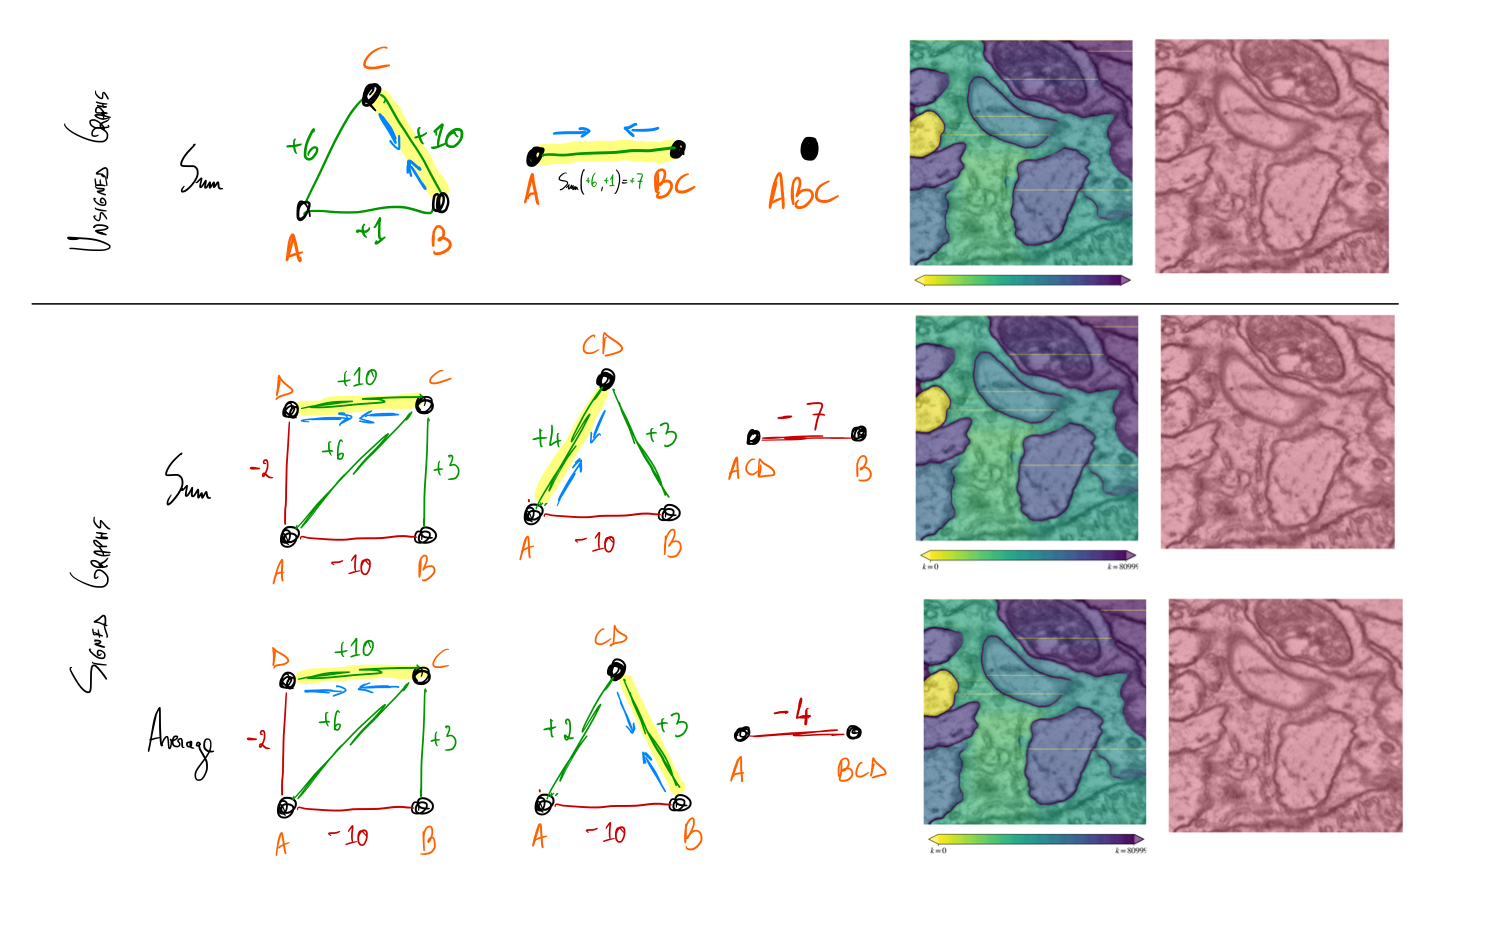
\includegraphics[width=0.5\textwidth,trim=0.4in 1.2in 0.in 0.05in,clip]{./figs/intro_image.jpg} % left bottom right top
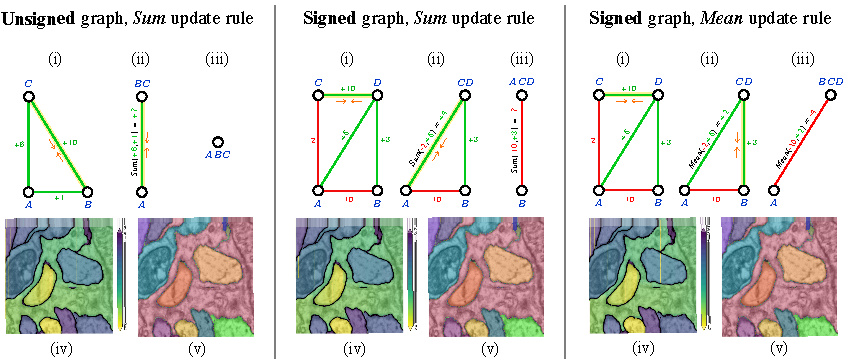
\includegraphics[width=\textwidth]{./figs/intro_image.pdf} % left bottom right top
\caption{
 (\textbf{a}) Iterations of three different algorithms in the generalized framework on  toy graph examples with attractive (green) and repulsive (red) interactions. (\textbf{b}) Example of CREMI 2016 neuron-segmentation data \cite{cremiChallenge} overlaid with instance segmentation. (\textbf{c}) Agglomeration order, representing which pairs of neighboring pixels were merged first (white), later on (brown), or never (black).
 \TODO{re-arrange, show affinities and replace unsigned case with Abs Max}
%We note how similar linkage criteria, like \emph{Sum} (in the middle) and \emph{Average} (on the right), lead to strongly different merging orders. 
% On the left: a single cluster is returned with only attractive interactions.
 % main ideas and contributions
\label{fig:intro_figure}}
\end{figure}
